\documentclass[tikz,border=5mm,12pt]{standalone}
\usepackage[fontsize=16pt]{fontsize}
\usetikzlibrary{arrows.meta}
\usetikzlibrary{calc}
\usetikzlibrary{positioning}

\begin{document}
  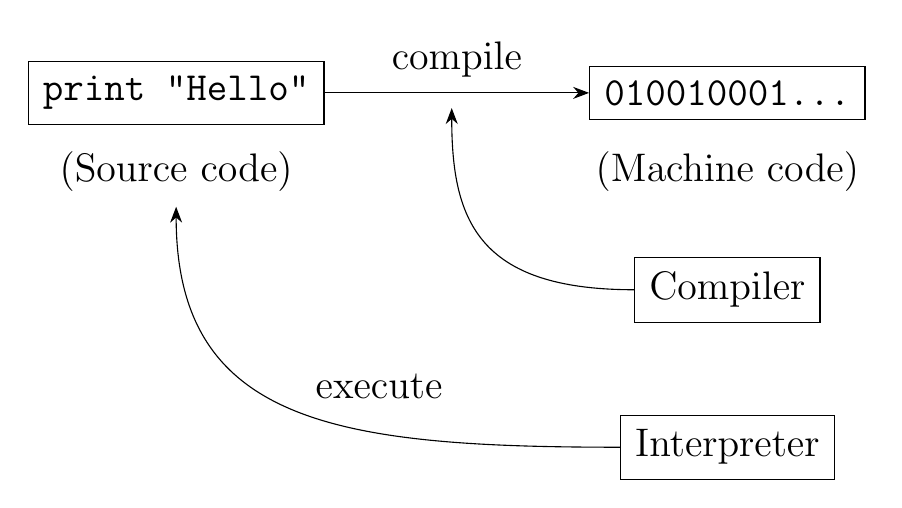
\begin{tikzpicture}[
    arrowtip/.style={
      -{Stealth[scale=1.2]}
    }
  ]
    \coordinate (AA) at ( 0mm,  0mm);
    \coordinate (AB) at (70mm,  0mm);
    \coordinate (BB) at (70mm,-25mm);
    \coordinate (CB) at (70mm,-45mm);

    \node[draw] (AAT) at (AA) {\small\texttt{print "Hello"}};
    \node[below of=AAT] (AAL) {\small (Source code)};

    \node[draw] (ABT) at (AB) {\small\texttt{010010001...}};
    \node[below of=ABT]       {\small (Machine code)};

    \node[draw] (BBT) at (BB) {\small Compiler};

    \node[draw] (CBT) at (CB) {\small Interpreter};

    \draw[arrowtip] (AAT.east) to (ABT.west);
    \path           (AAT.east) -- (ABT.west) node[midway,above] {\small compile};
    \path           ( AA.east) -- ( AB.west) node[midway] (ABM) {};

    \draw[arrowtip] (BBT.west) .. controls +(180:20mm) and +(-90:16mm) .. (ABM);

    \draw[arrowtip] (CBT.west) .. controls +(180:36mm) and +(-90:32mm) .. (AAL);
    \path           (CBT.west) --                                         (AAL)
      node[midway,below,xshift=-6mm,yshift=-4mm] {\small execute};
  \end{tikzpicture}
\end{document}
